\begin{figure}[bp!]
  
  \centering
  \caption{An example of a bar graph}
  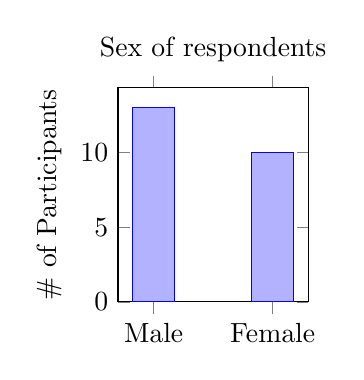
\begin{tikzpicture}
    \begin{axis}[
      title={Sex of respondents},
      ybar,
      bar width=15pt,
      enlarge x limits=0.3,
      ylabel={\# of Participants},
      symbolic x coords={Male,Female},
      xtick=data,
      ymin=0,
      width=4cm,
      height=4.3cm,
    ]
    \addplot coordinates {(Male,13) (Female,10)};
    \end{axis}
  \end{tikzpicture}

\end{figure}